% !TEX root = ../thesis.tex
\documentclass[thesis.tex]{subfiles}
\begin{document}



\chapter{Background}
\label{chapter:background}

This chapter provides an introduction to concepts that help understand how smartphones and photoluminescence can be applied for product authentication purposes. Chapter \ref{section:existing_solutions} presents an overview of existing smartphone-based product authentication solutions. Chapter \ref{section:photoluminescence} continues with an introduction to photoluminescence and its applications. Chapter \ref{section:rgbhsv} discusses three widely adopted color models (RGB, HSV and YCbCr) and their distinct application areas. Chapter \ref{section:mobile_camera_technology} will first discuss the color image pipeline of a camera to provide a better understanding of the recent mobile camera innovations introduced later in the chapter. Last, Chapter \ref{section:hybrid_mobile_landscape} covers the hybrid mobile landscape, the different ways of developing hybrid applications (WebView app and Compiled Hybrid app) and how they compare to fully native solutions. The focus will be on WebView apps while an overview of different Compiled Hybrid app solutions will be provided towards the end of the chapter.

\clearpage

\section{Existing Solutions}
\label{section:existing_solutions}

A wide spectrum of technologies exist for product authentication purposes. Existing solutions range from the use of inexpensive seals and electronic labels to carefully crafted watermarks and even DNA. These technologies can be categorized, for example, by their level of security, cost and portability. The focus of this chapter is on commercial smartphone-based product authentication solutions that often trade high precision (or reliability) for better cost-efficiency and portability. These solutions can be considered as competition for the technology explored in this thesis. An overview of a number of different product authentication technologies and their background is given in \cite{kuosmanen}.

InkSure's SmartSure technology authenticates products by utilizing a chemical marker (taggant) embedded in a hologram. The authenticity of the taggant is verified by capturing an image of the hologram and sending it to a cloud platform for further processing. The platform also offers track-and-trace reporting services. The smartphone application uses a QR scanner and visual aids to help the user position the viewfinder properly over the hologram. \cite{inksure} An example of SmartSure's user interface can be seen in Figure \ref{figure:inksure}.

\begin{figure}[ht]
\centering 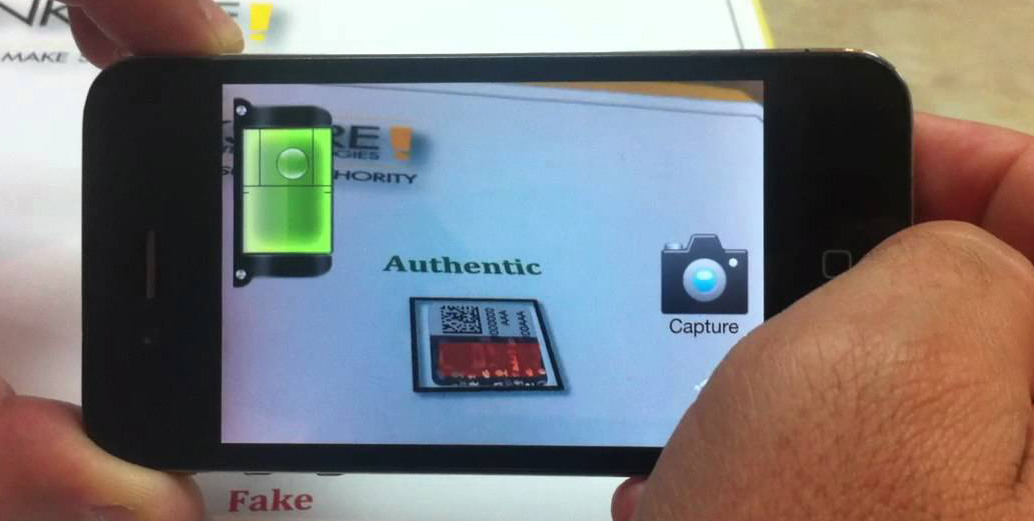
\includegraphics[width=13.25cm]{images/existing_solutions/smartsure}
\caption{InkSure's SmartSure iPhone application UI. The red rectangle and a virtual spirit level are used to position the smartphone correctly. \cite{inksure} \label{figure:inksure}}
\end{figure}

AlpVision and its CryptoGlyph\textregistered\ technology takes a very different approach. CryptoGlyph\textregistered\ makes use of a pseudo-random pattern of tiny dots (40-80 microns) printed on the coating of a material. The color and size of the dots are customized based on the packaging color. The authenticity of a product is verified by matching a pattern on the product to a pattern stored in a remote database. As of this writing AlpVision's iOS and Android applications are not publicly available in their respective application stores, but instead distributed as tailored applications ``to meet the client's unique authentication needs''. Figure \ref{figure:alpvision} illustrates how differently sized and color dots affect their visibility and how they are applied to the coating of a material. \cite{alpvision}

\begin{figure}[hb]
\centering 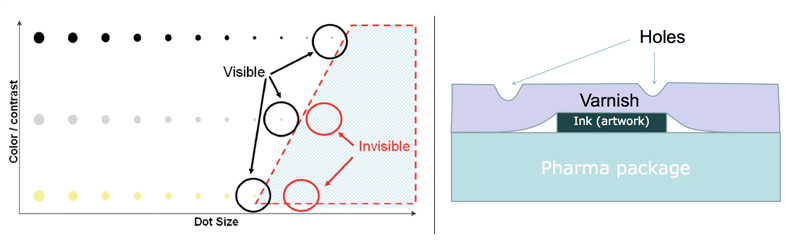
\includegraphics[width=\textwidth]{images/existing_solutions/cryptoglyph}
\caption{AlpVision's CryptoGlyph\textregistered\ embeds micro-dots on the coating of a material to create unique invisible patterns for product authentication \cite{alpvision}. \label{figure:alpvision}}
\end{figure}

The growing number of NFC-enabled phones in the market (estimated to have reached 53\% of the overall market in 2015 according to \cite{frost-sullivan}) has given companies the incentive to utilize NFC-based technologies for product authentication purposes. Secure and specialized NFC tags have been manufactured by a number of companies since the technology was first introduced to the market in 2006. However, only few companies have developed the software and services exclusively for NFC-based product authentication. Examples of such companies include FinnCode\footnote{\url{http://www.finncode.com/}} and Selinko\footnote{\url{http://selinko.com/}}, which manufacture their own secure NFC tags and offer a SaaS-based product authentication platform for their clients. Other notable smartphone powered product authentication applications include scryptoTRACE\textregistered\ by U-NICA, CertiEye by Infotoo and AuthentiGuard by DSS. A summary of the different solutions is provided in Table \ref{table:existing-solutions} for comparison.

\begin{table}[ht]
	\caption{Existing solutions for smartphone-based product authentication.} \label{table:existing-solutions}

	\begin{center}
	\begin{tabular}{| m{2cm} | m{3.25cm} | m{3cm} | m{3.75cm} |}

		\hline
		\textbf{Company}				&	\textbf{Product name}			&	\textbf{Platforms}			&	\textbf{Technologies} \\ \hline
		InkSure\newline (American)		&	SmartSure						&	iOS							&	Chemical taggant,\newline hologram \\ \hline
		U-NICA\newline (Swiss)			&	scryptoTRACE\textregistered		&	iOS, Android				&	Micro-printing,\newline edge detection \\ \hline
		AlpVision\newline (Swiss)		&	CryptoGlyph\textregistered		&	Customized\footnotesize{*}	&	Micro-printing,\newline pattern recognition \\ \hline
		DSS\newline (American)			&	AuthentiGuard					&	Customized\footnotesize{*}	&	Undisclosed \\ \hline
		Infotoo\newline (Chinese)		&	CertiEye						&	iOS, Android				&	Undisclosed \\ \hline
		FinnCode\newline (Finnish)		&	FinnCode\newline Authentication			&	iOS, Android				&	NFC \\ \hline
		Selinko\newline (Belgian)		&	Selinko							&	Android						&	NFC \\
		\hline
	\end{tabular}
	\end{center}
	\scriptsize{*} \small{privately distributed, the application is developed according to the client's needs.}
\end{table}

\section{Photoluminescence}
\label{section:photoluminescence}

Photoluminescence, one of the many forms of luminescence (light emission), is a process where a substance absorbs photons (light) and emits back a certain wavelength of light. Based on the lifetime of the emission (decay time) photoluminescence can be more specifically referred to as \emph{fluorescence} or \emph{phosphorescence}. Fluorescence is typically measured in nanoseconds (from absorbtion to emission) whereas the duration of phosphorescence is anything from a few milliseconds to seconds or even hours \cite{luminescence_basics}. Materials that have \emph{photoluminescent} properties are typically referred to as \emph{luminophores} (or respectively, as fluorophores or phosphors).

Figure \ref{figure:photoluminescence} illustrates the process of photoluminescence. The first phase of photoluminescence is \emph{photoexcitation}, the absorption of photons causing an electron to move to a higher energy state ($S_0 \rightarrow S_2$). The absorption is followed by internal conversion (IC), where the electron transitions within picoseconds from a higher energy state to a lower energy state. After the electron has reached the lowest excited energy state ($S_1$) it relaxes, eventually reaching the the ground state ($S_0$). This occurs either directly as a rapid emission of light (fluorescence) or through a so called intersystem crossing (ISC) resulting in a relatively slow emission of light as the electron travels from one state to another (phosphorescence).

\begin{figure}[hb]
\centering 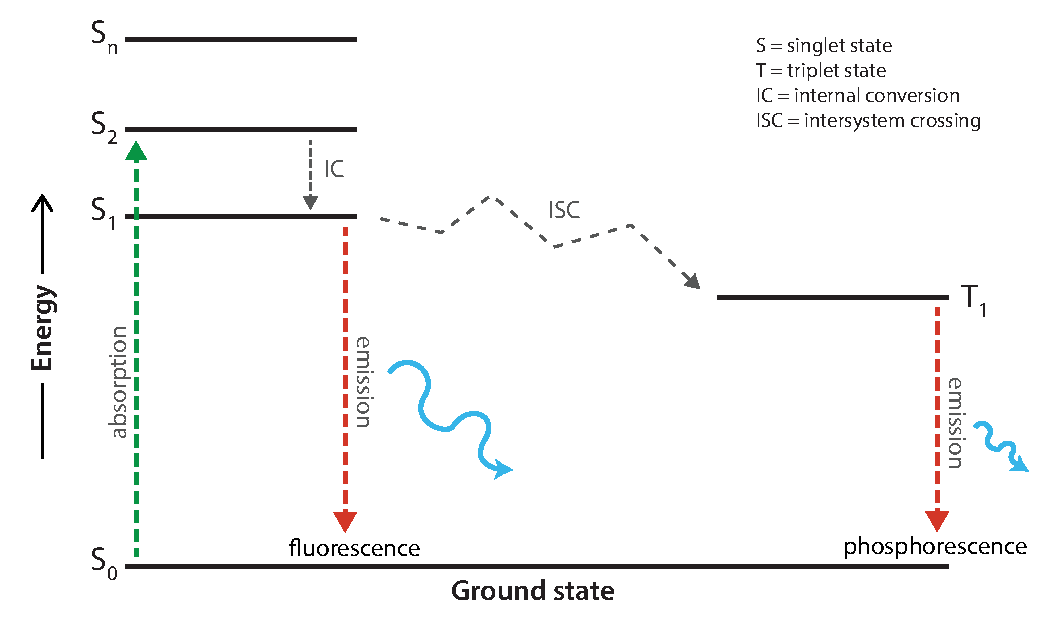
\includegraphics[width=\textwidth]{images/photoluminescence.pdf}
\caption{A simplified Jablonski diagram of photoluminescence. \label{figure:photoluminescence}}
\end{figure}

\noindent Since the energy of the electron at the triplet state is lower than at the singlet state phosphorescence typically occurs at longer wavelengths of light than fluorescence. Furthermore, phosphors have a longer \emph{excited state lifetime} as the relaxation from the triplet state ($T_1$) to the singlet state ($S_0$) is kinetically unfavorable, and thus, occurs at a much slower pace. Due to the longer lifetime phosphors typically emit light long after the initial absorption of photons. \cite{CEJ}

Luminophores always emit longer wavelengths (less energy) than what they absorb. This is due to the loss of energy within the emission pathway. For example, during the IC and ISC transitions some of the excitation energy transforms into heat. The difference between the absorption and emission wavelength is known as the \emph{Stokes shift}. The magnitude of Stokes shift depends on the chemical properties of the luminophore. For fluorophores it is typically in the range of 30-50 nanometers while for phosphors, such as Lanthanide Chelates, it can range up to 200 nanometers. Luminophores are also subject to different environmental effects: changes in temperature, pH, concentration or the amount of dissolved oxygen in the compound affect the intensity of the luminophore and can even shift its natural emission wavelength \cite{hemmila}. \cite{luminescence_basics} \todo{citation ordering?}

\begin{figure}[ht]
\centering 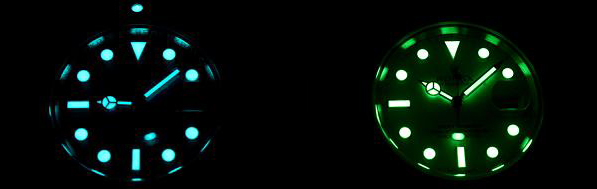
\includegraphics[width=\textwidth]{images/photoluminescence_example}
\caption{An illuminated watch face is a typical commercial application of photoluminescence. More expensive watches typically use radioluminance and a radioactive substance like tritium for a similar effect.\label{figure:photoluminescence_example}}
\end{figure}

Photoluminescence has many applications areas. It can be used for forensic analysis, to detect impurities in a system, or to study structures \cite{photoluminescence_use_case_2}\cite{photoluminescence_use_case_1}\cite{photoluminescence_use_case_3}. This is typically achieved through \emph{luminescence spectroscopy}, which provides a non-destructive and non-invasive manner to study materials. In commercial products luminescence is often used for illuminating watch faces under poor lighting conditions as illustrated in Figure \ref{figure:photoluminescence_example}. Phosphor-coated elements of a watch face exposed to bright daylight continue to glow in the dark for the duration of the phosphorescence. More expensive watches utilize radioactive substance enclosed within the phosphor coating to excite the electrons with radiation instead of depending on an external light source. This form of luminescence is known as radioluminescence.

\section{Color Models}
\label{section:rgbhsv}

A wavelength of light (emitted for example by a luminophore) falling within the visible spectrum of the human eye (\mytilde390-700nm) creates a perception of color. Color models are used to represent this perception in a medium by providing an abstract mathematical model for describing colors numerically, typically as a vector of 3 or 4 dimensions. A color model alone is only sufficient for relative comparison of colors within that particular model. It is not until the model is given a \textit{context} that it forms a \textit{color space} and the relative colorimetric values map to their absolute counterparts. Here context denotes a set of external (standardized) viewing conditions, in which the colors are expected to be rendered. For example, the standard sRGB color space is based on the RGB color model and assumes an ambient illuminance of 64lux as per IEC \cite{iec}. The term color model is sometimes referred to as \textit{non-absolute color space} or \textit{relative color space} even if it were less ambiguous to limit the discussion to color models (relative) and color spaces (absolute).

\subsection{RGB}
RGB is the most common color model found in today's computer displays and monitors. It is largely influenced by the historical research on human color vision: the Young–Helmholtz theory of trichromatic color vision, formulated in the 18th century, proposed that color vision is the result of three different photoreceptor cells (cone cells). Later, in 1956 this theory was backed by psychological evidence, which showed that the human retina is particularly sensitive to three groups of wavelengths in the areas of blue, green and red. \cite{svaetichin}

RGB is an \textit{additive} color model, which means that RGB colors are produced by adding together two or more primary colors: red, green or blue. All RGB colors are defined relative to these three primary colors and adding them all together yields white. Respectively, the color of pure yellow would contain all the red and green but no blue: RGB(100\%, 100\%, 0\%).

Like all color models, RGB itself does not specify what is meant by red, green and blue colorimetrically. That is the purpose of color spaces, such as sRGB, which define the exact values (chromaticities) for the RGB primaries, typically in terms of so called \textit{tristimulus values} (X, Y and Z). The tristimulus values correspond to a color in the \textit{CIE x-y chromaticity diagram}, which has been established \emph{through empirical research} to represent all of the chromaticities visible to the average human eye \cite{cie}. A given color space can only produce the colors that fall within its \textit{gamut}, the triangle defined by the chromaticities of its primaries as illustrated in Figure \ref{figure:srgb}. As RGB has been found to model the human color vision reasonably accurately, sRGB has become the standard color space for today's digital consumer products. However, for some use cases there exists better alternatives, which are covered in more detail in the following chapters.

\clearpage
\begin{figure}[ht]
\centering 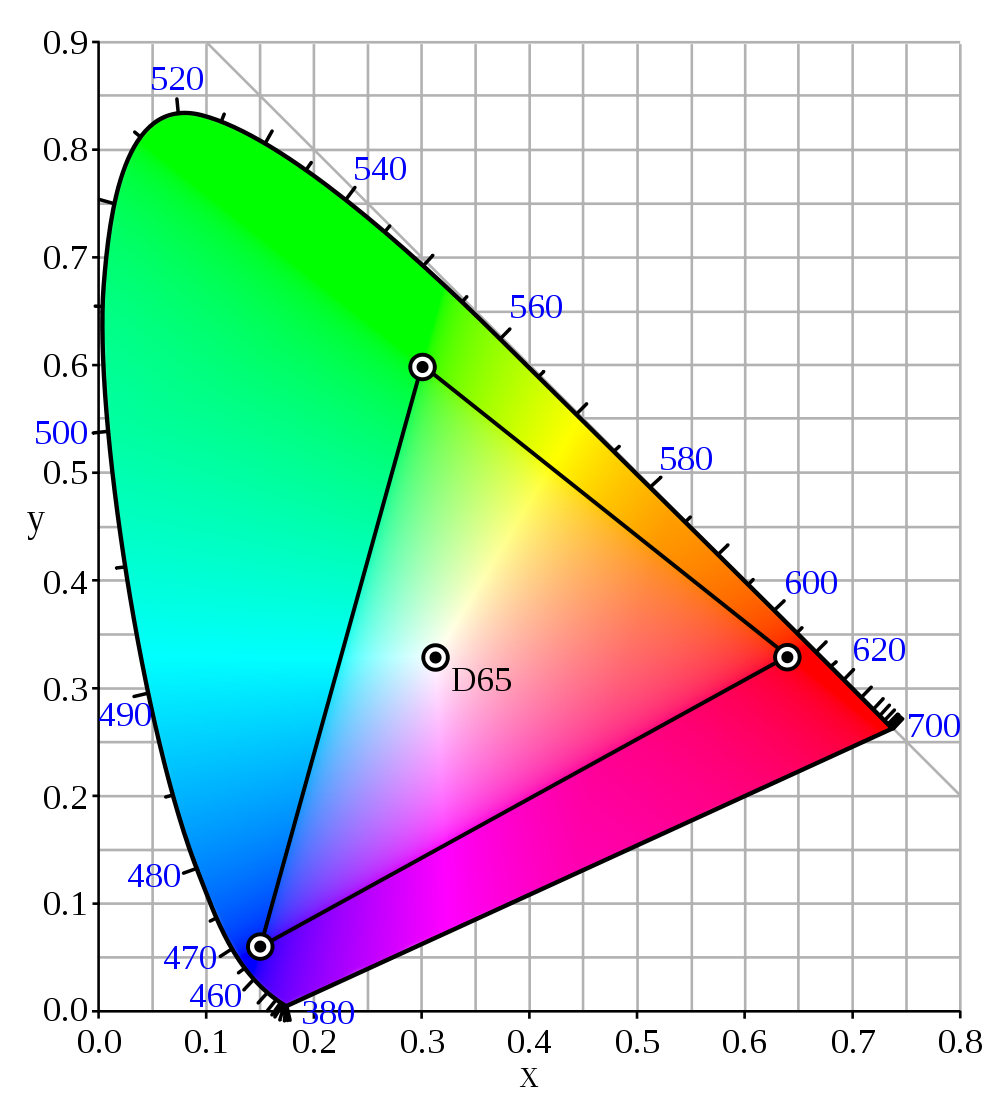
\includegraphics[width=0.75\textwidth]{images/srgb}
\caption{The CIE x-y chromaticity diagram and sRGB gamut (triangle). A color space can only render the subset of colors that are within its gamut.\label{figure:srgb}}
\end{figure}

\subsection{HSV}

HSV (hue-saturation-value) color model was developed in the late 1970s in an attempt to create a more intuitive and perceptually relevant color model for different computer graphics applications. HSV rearranges the cartesian geometry of RGB to a cylindrical coordinate system separating the color information (chroma) from the brightness information (luma). The geometrical representations of RGB and HSV are depicted in Figure \ref{figure:rgb_hsv} for comparison.

The ability to decouple luma from chroma brings many benefits for graphics processing applications. Many common computer vision algorithms designed for grayscale images, such histogram equalization, canny edge detection or binary thresholding, become trivial in HSV space as the grayscale information can be read directly from the luma component (V) \cite{color_segmentation}. HSV has also become the de facto model for color pickers as the relationship between hue, saturation and brightness are both conceptually and perceptually easier to reason about than that of red, green and blue.

\begin{figure}[ht]
\centering 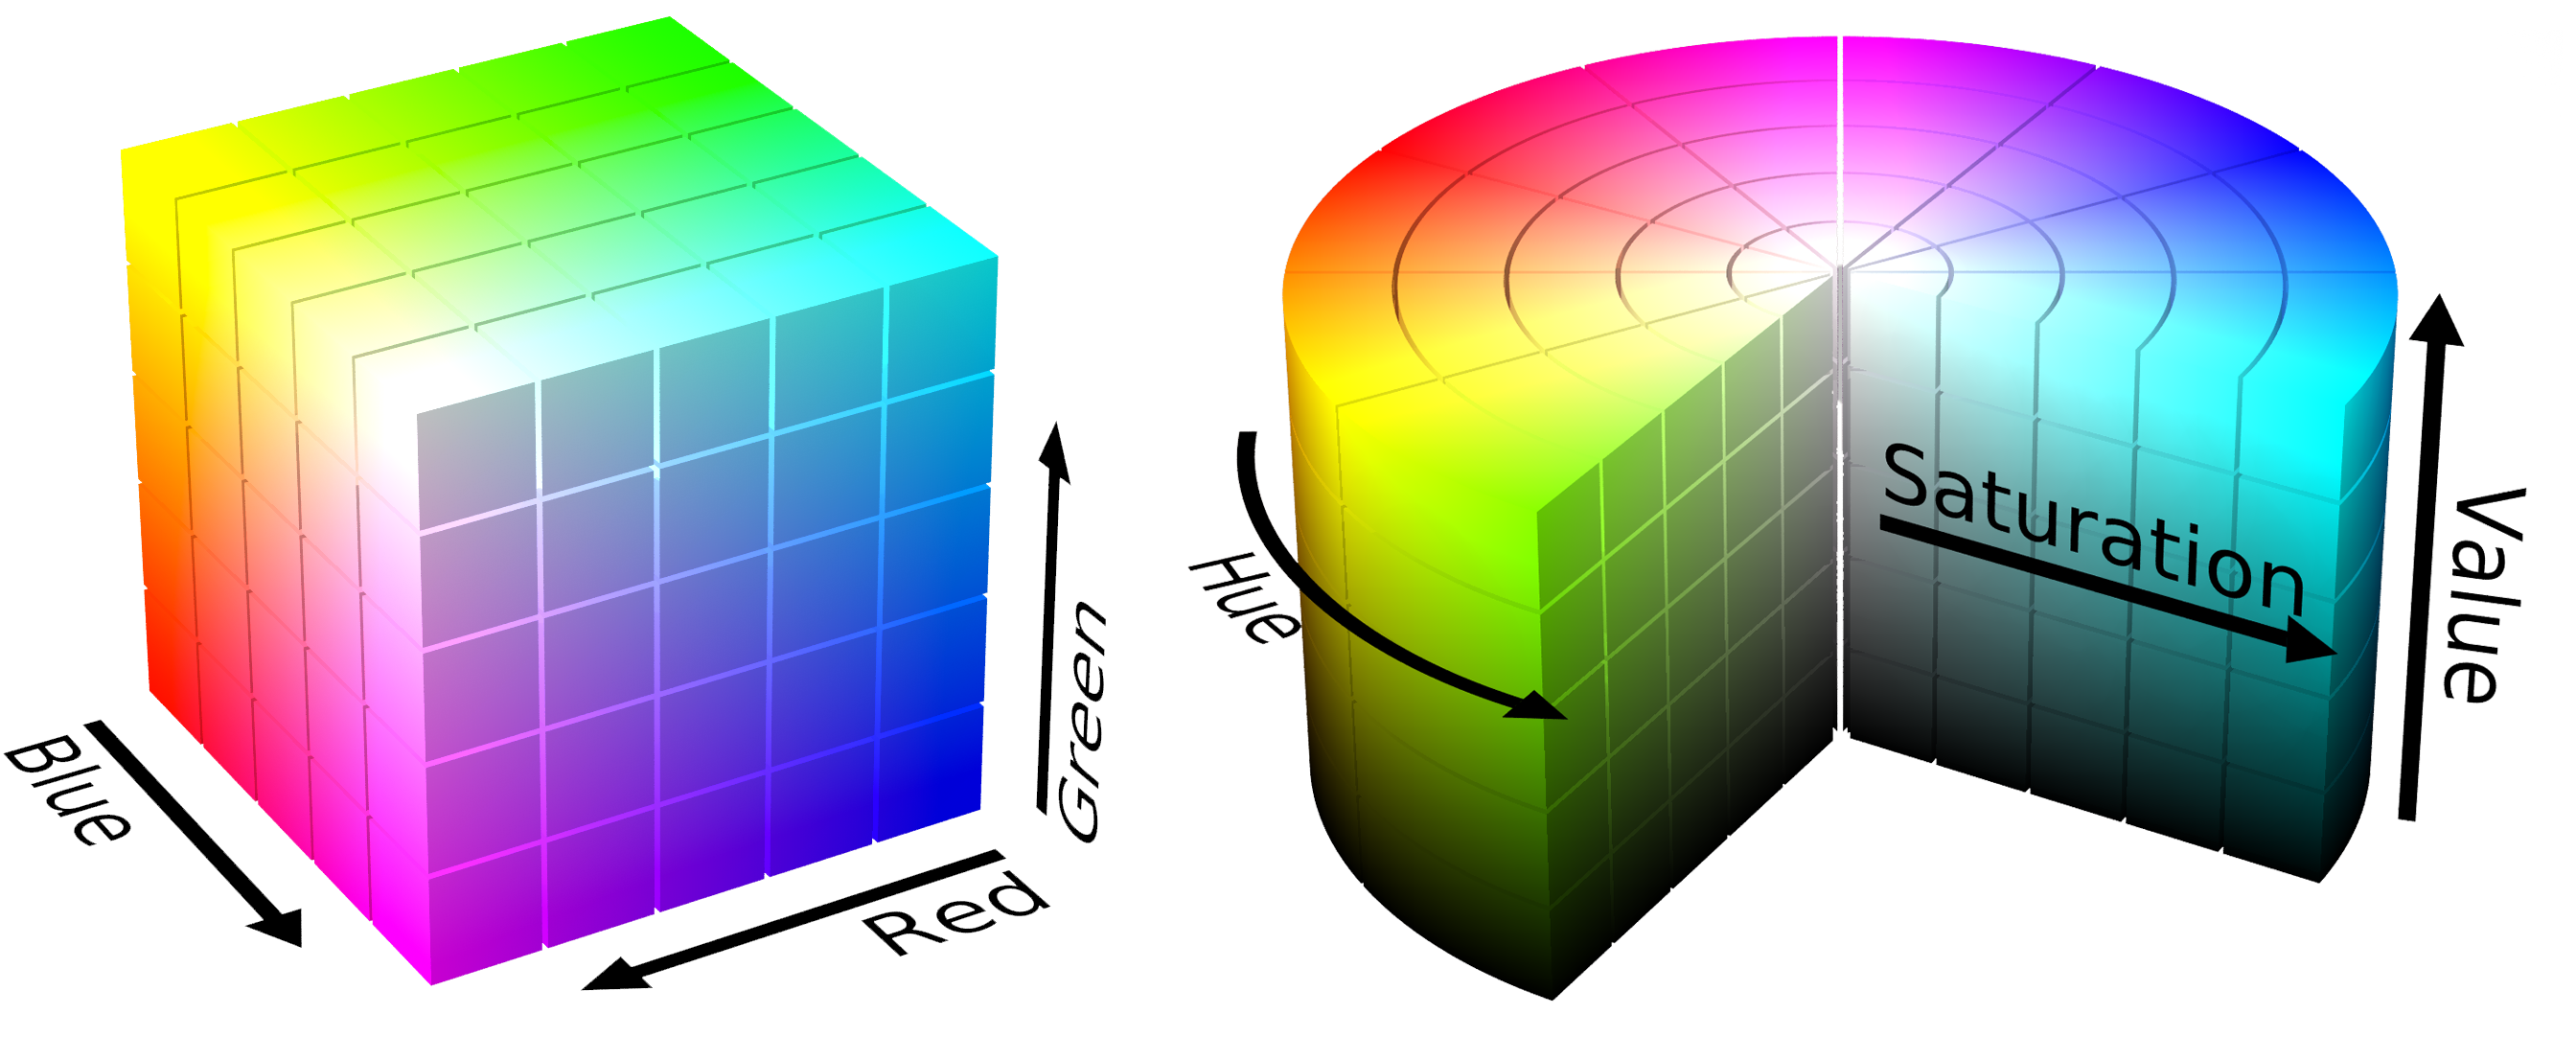
\includegraphics[width=\textwidth]{images/rgb_hsv}
\caption{RGB colors are typically presented in cartesian coordinates whereas HSV colors use cylinder coordinates \cite{hsv_cylinder}\cite{rgb_cube}.\label{figure:rgb_hsv}}
\end{figure}

RGB values can be converted into HSV using a simple linear transformation. The formal definition of the transformation is given by the following formula:

\begin{align}
\label{rgb-to-hsv}
V &\leftarrow C_{max}	&
S &\leftarrow
	\begin{cases}
		\frac{C_{delta}}{C_{max}}, & \text{if $V\neq0$}\\
		0, & \text{otherwise}
	\end{cases}			&
H &\leftarrow
	\begin{cases}
		\frac{60(G-B)}{C_{delta}}, & \text{if V=R}\vspace{2mm}\\
		\frac{120+60(B-R)}{C_{delta}}, & \text{if V=G}\vspace{2mm}\\
		\frac{240+60(R-G)}{C_{delta}}, & \text{if V=B}
	\end{cases}
\end{align}
\noindent where
\begin{flalign*}
&C_{max}=max(R, G, B),\\
&C_{delta}=max(R, G, B) - min(R, G, B),\\
&R, G, B = \{\ x\ \vert\ x \in \mathbb R\ \wedge\ 0 \leq x \leq 1\ \}.
\end{flalign*}

\subsection{YCbCr}
YCbCr (or YCC) is a family of color spaces used as a part of the color image pipeline of video and digital imaging systems. YCbCr was primarily developed as an intermediate format enabling a way of storing and transmitting color information with minimal redundancy. Much like HSV it separates luma (Y) from chroma (Cb and Cr) but also compresses the chroma components for improved storage and transmission capabilities. Because the human visual system has lower acuity (sensitivity) for changes in color than luminance, the signal can be optimized by compressing the color components resulting in no perceptible loss in quality. \cite{color_vision}

\begin{figure}[h]
\centering 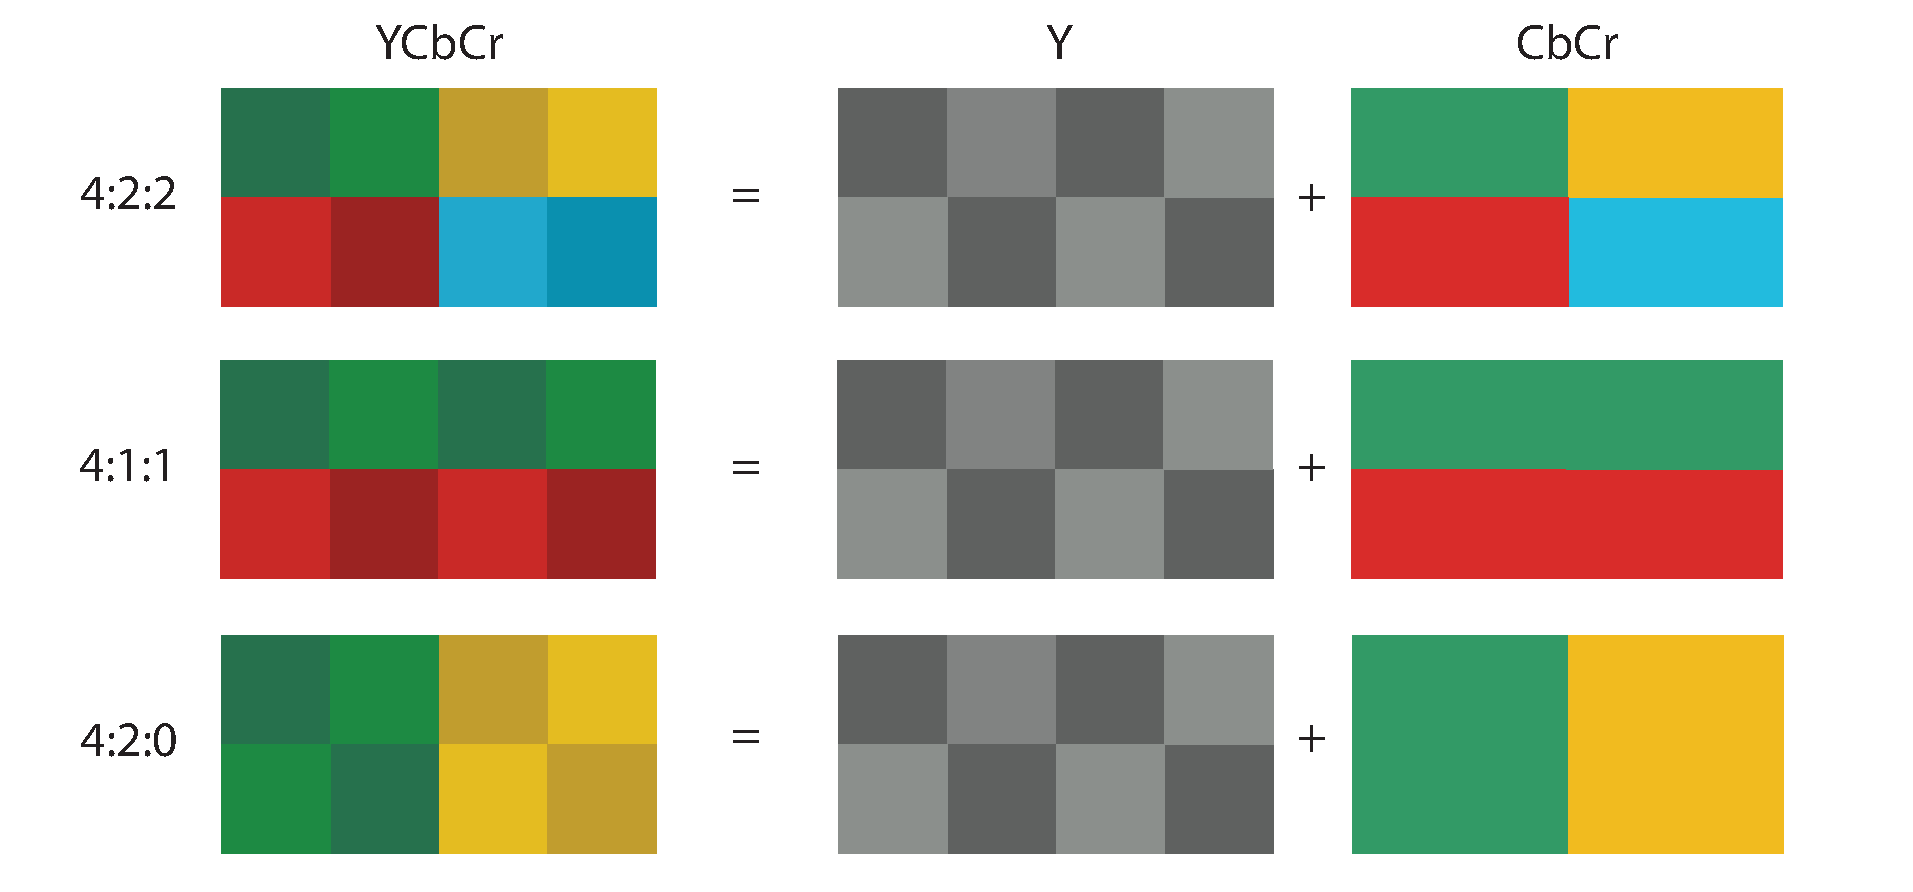
\includegraphics[width=\textwidth]{images/ycbcr}
\caption{Different YCbCr schemes subsample chroma in various ratios.\label{figure:ycbcr}}
\end{figure}

Each YCbCr format uses different subsampling scheme for the compression. Figure \ref{figure:ycbcr} illustrates the most common YCbCr subsampling (or chroma subsampling) ratios: 4:2:2, 4:1:1 and 4:2:0. The last two digits denote at which ratio the chrominance information is encoded. For example, in the 4:2:0 format both the horizontal and vertical resolution of the Cb and Cr chroma components are halved and stored in adjacent columns resulting in a 50\% reduction in required bandwidth. Different YCbCr schemes can offer the same level of compression (e.g. 4:2:0 and 4:1:1). The appropriate format is typically selected based on the format the target medium supports in order to avoid the need for any subsequent conversions.

\section{Mobile Camera Technology}
\label{section:mobile_camera_technology}
Mobile camera technology has evolved at an increasing pace ever since the early 2000s when the first camera phones arrived in the market. The main driving force behind the rapid development has been the competition for customers and emerging markets in Asia and Africa. Much like traditional point-and-shoot cameras, most commerical smartphones are often marketed largely by their features to attract the masses. Megapixels, higher shutter speeds, better zooming capabilities and features like High Dynamic Range photography (HDR) have cought the interest of customers but also pushed the limits, within which mobile and camera manufacturers operate. And, unlike in the case of more traditional Digital Still Cameras (DSC), manufacturers are met with further physical (size) and practical (cost and power consumption) constraints as cameras are just one of the many basic features of today's smartphones.

\subsection{Image Pipeline}
Before an image is ready to be rendered or stored in a medium it goes through a series of processing steps commonly referred to as the image pipeline. The image pipeline in modern smartphones is very similar to that of typical DSCs. However, due to higher price pressure and limitations in available space and power, smartphone manufacturers need to compromise. To maximize available space some of the processing is often moved from hardware to software, while costs are kept low by using components of lower quality. The implementation of the pipeline depends on the manufacturer and the complexity of the camera module.

Figure \ref{figure:pipeline} illustrates the different stages of a typical image pipeline. The light reflected from a scene travels through the camera's lens system and an array of filters before hitting the sensor. The pixels (photosites) of the sensor capture the incoming light (photons), which the sensor turns into voltage. The Analog-to-digital converter (ADC) is responsible for converting the voltage into a digital representation. Finally, the signal reaches the Image Signal Processor (ISP), which applies a host of different image processing techniques to construct the final image before it is transmitted to the medium for display and storage. Like most commercial DSCs smartphone cameras favor the CMOS sensor technology for its better cost and energy efficiency over the more historical CCD technology.

\begin{figure}[h]
\centering 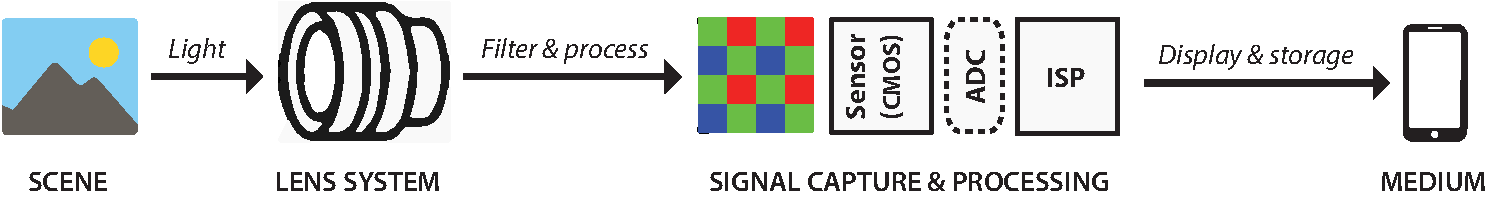
\includegraphics[width=\textwidth]{images/pipeline}
\caption{The different stages of a typical color image pipeline.\label{figure:pipeline}}
\end{figure}

The amount of light falling on the sensor is controlled by the camera's exposure settings. The three factors that affect exposure are aperture, shutter speed and ISO sensitivity. Aperture defines the effective diameter of the lens opening in terms of a so called \textit{f-number} --- the smaller the f-number the wider the opening. Smartphone cameras typically have a fixed aperture lens with a low f-number (f/2.0 - f/2.4). The motivation for using wide fixed apertures is twofold. First, a fixed aperture lens requires less parts and space than a lens of variable aperture lowering the costs and complexity of the pipeline. Second, a wide aperture allows for more light to fall on the smartphone's relatively the small sensor.

Longer shutter speeds allow more light to be captured whereas a higher ISO increases the sensor's ability (sensitivity) to collect more photons. However, long shutter speeds are often not suitable for capturing moving objects due to image blur. High ISO values on the other hand affect the quality of the image by introducing noise. Smartphone cameras are typically equipped with an electronic shutter, since it is more cost-effective, faster and has less lag than a mechanical shutter. However, the required extra circuitry around the sensor makes the system more prone to noise due to interference. As of this writing, support for manual exposure control is still relatively poor. Android 5, iOS8 and Windows Phone 8.1 were the first smartphone OS releases to introduce camera APIs that would support manual control over shutter and ISO speeds.

The lens system and filters laid over the sensor also affect the incoming light. A lens system comprises multiple stacked lenses that correct different geometrical and chromatic aberrations such as vignette, coma, barrel and pincushion distortion. Since smartphone camera lenses have both a fixed aperture and focal length these aberrations can be corrected easily. Once the light has travelled through the lens system and before it reaches the sensor it is anti-aliased, filtered for infrared and colour sampled using a Color Filter Array (CFA). \cite{color_pipeline}

The purpose of a CFA is to help the sensor filter different wavelengths of the incident light. As the sensor itself is only capable of capturing intensities it is overlaid by a CFA so that a given pixel will capture only particular wavelengths of light. The most common CFA is the \textit{Bayer filter}, which is found in most of today's smartphones and consumer level DSCs. The Bayer filter consists of alternating rows of red-green and green-blue color filters as illustrated in Figure \ref{figure:bayer}. Since the human eye is more sensitive to green light than red or blue the Bayer filter has twice the number of green filters as red or blue. The Bayer filter discards roughly 2/3 of the incident light as each pixel can only capture the intensity of one of the three primary colors (wavelengths).

\begin{figure}[h]
\centering 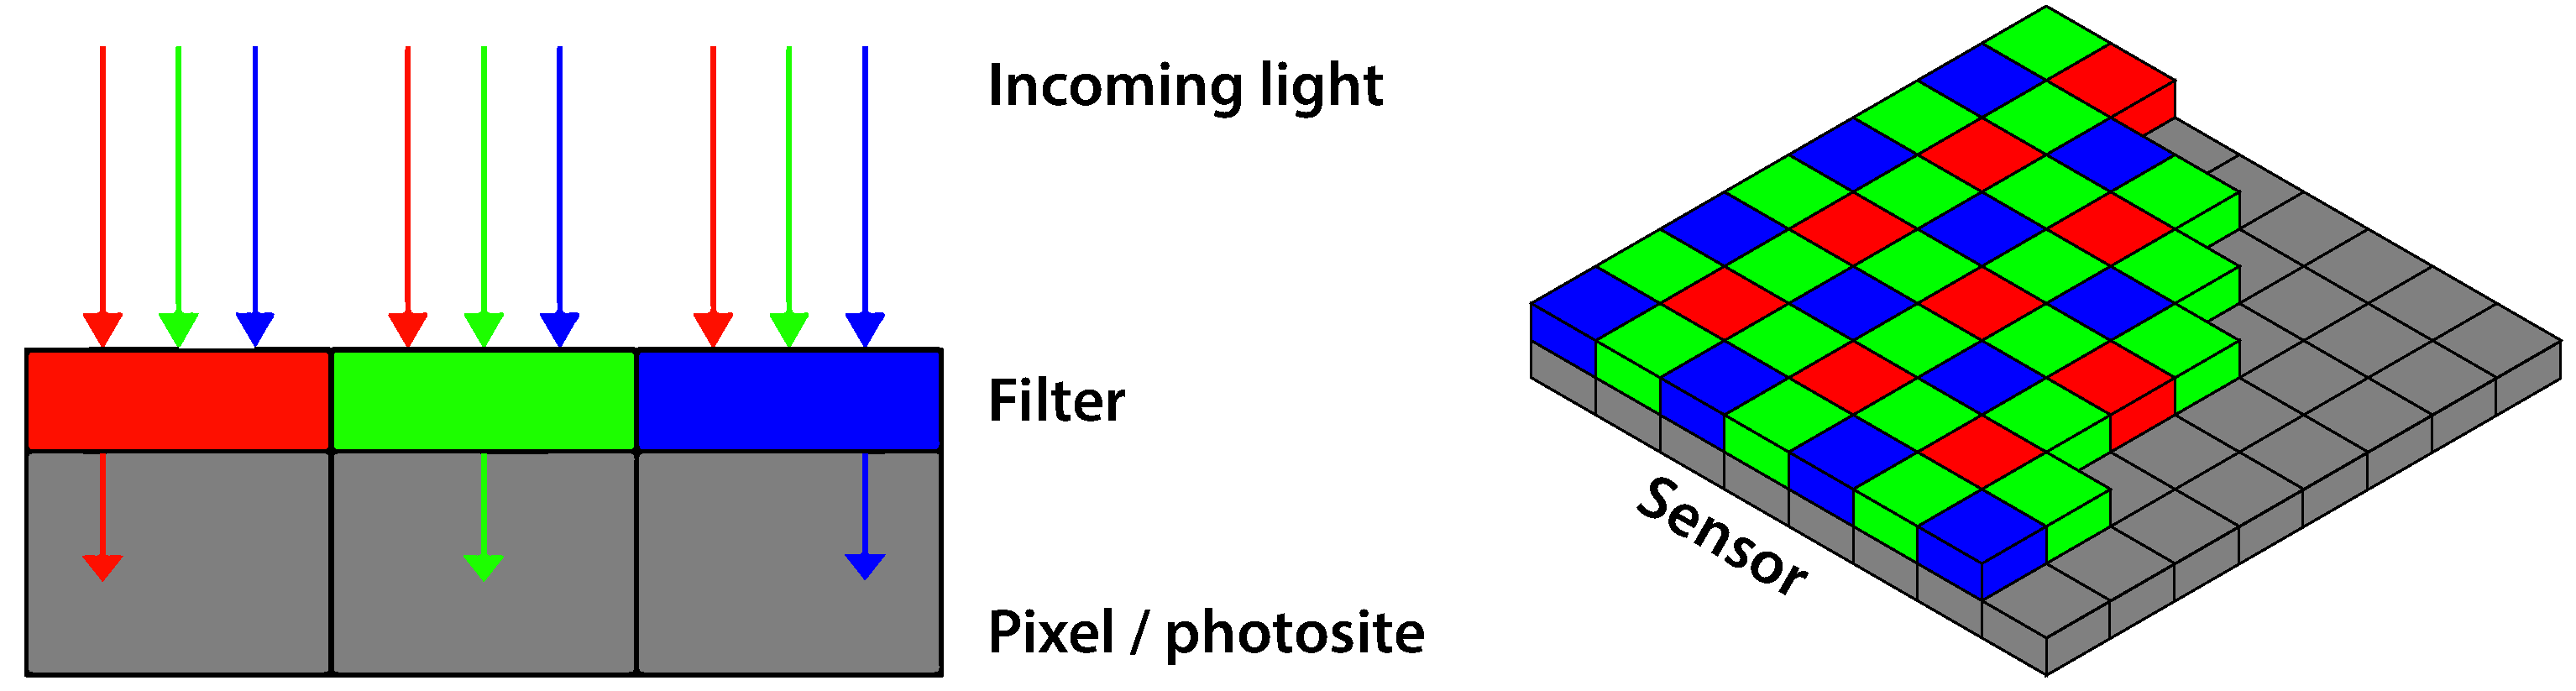
\includegraphics[width=\textwidth]{images/bayer}
\caption{The Bayer filter filters the incident light into intensities of red, green and blue color, which are then interpolated to construct the final image. \label{figure:bayer}}
\end{figure}

The filtered output of the sensor is reconstructed into a full color image by the ISP. This process is commonly denoted as \textit{demosaicing} or CFA interpolation, and is typically preceded and followed by different image processing techniques such as white balance adjustment, image sharpening and noise reduction. The exact order in which these processes are applied and the type of algorithms used are manufacturer secrets and an active area of competition. The pixel data is typically encoded in RGB, or alternatively, in a compressed format like YCbCr. Some high-end smartphones, like Nokia 1020 and Nexus 6, are able to store the unrendered sensor data, often referred to as RAW. The benefit of RAW format is that it allows color corrections to be made in a wide-gamut color space (e.g. Adobe RGB) before converting the data to a rendered color space of the output media (e.g. sRGB). Most smartphones store RAW data in the lossless Digital Negative format (DNG).

\subsection{Recent Developments}\label{chapter:solutions}

Smartphone cameras are slowly evolving from simple snapshot instruments to devices offering near professional quality image capturing capabilities. The first steps towards this trend were taken during 2012-2013 when Nokia released its first PureView powered phones, Nokia 808 and Nokia 1020. They were the first commercially available smartphones to include sensors bigger than most mid-level compact cameras featuring form factors more than twice the size of the typical 1/3" sensor found in most today's smartphones (1/1.2" and 1/1.5" respectively). The Nokia's PureView technology utilizes the camera's relatively large sensor size to provide \textit{lossless zoom} by means of oversampling. For example, cropping the 41MP image of Nokia 1020 down to 5MP (A3 size) yields a magnification factor of 3 without a perceivable loss in quality. Moreover, cropping the image around its center has the benefit of mitigating many common aberrations such barrel distortion and vignette. \cite{lumia_1020}

Another new technology featured in the Nokia 1020 was back-illuminated sensor (BI). After the first BI powered smartphones appeared in the market in 2010 (HTC Evo 4G) and 2011 (Apple iPhone 4) the technology has seen wide adoption, especially in high-end smartphones. BI is a technology targeted for improving the sensitivity of CMOS sensors. While the more traditional front-illuminated CMOS sensors are less expensive and easier to manufacture, BI sensors provide better image quality and light sensitivity by novel arrangement of imaging elements and circuitry underneath the sensor surface.

Recent innovations behind Nokia's flagship phones and other high-end mobile devices have mainly focused on optimizing existing hardware. Sony, however, has taken a different approach with its QX product line first released in late 2013. Sony's QX products include different \textit{smartphone attachable lens-style cameras}, which are mountable camera modules that can be used as a replacement for the smartphone's built-in camera (Figure \ref{figure:sony-qx}). The idea is similar to that of professional digital single-lens reflex cameras (DSLR), which allow different lenses to be mounted on the camera body. While the Sony QX camera modules have internal storage capabilities, they require a Wi-Fi connection for communicating with and transferring data to the smartphone.

\begin{figure}[h]
\centering 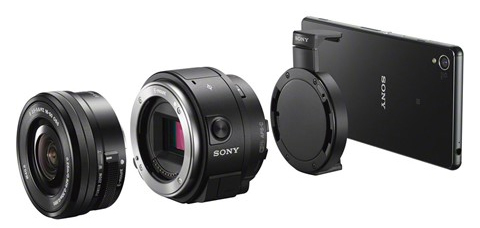
\includegraphics[width=\textwidth]{images/sony_qx.jpg}
\caption{Sony's interchangeable camera modules: QX10 lens camera (left) and QX30 lens mount (middle) featuring an APS-C size sensor.\label{figure:sony-qx} \cite{sony_qx}}
\end{figure}

In the near future Google's Project Ara aims to take \textit{smartphone modularization} a step further. The goal of the project is to offer a base smartphone model that can be customized and extended by interchangeable third-party components. For example, in low-light conditions less noisy images could be produced by mounting the base model with a camera module featuring bigger pixels or a wider aperture. The modular approach of Ara could also make smartphones a suitable platform for different computational photography applications as it would allow easier integration of specialized ISP chips like NVIDIA's Chimera\texttrademark or Movidius' Myriad processor.

Smartphone modularity has also been on Apple's radar as evidenced by patents they have acquired for interchangeable iPhone camera lenses \cite{apple_patent_camera_module_3}\cite{apple_patent_camera_module_4}\cite{apple_patent_camera_module_5}. Other future mobile camera technologies Apple is working on include multi-sensor camera and refocusable imaging mode \cite{apple_patent_camera_module_1}\cite{apple_patent_camera_module_2}. The patented multi-sensor system uses three separate sensors, one for luminance and two for chrominance, to produce images of higher resolution and color accuracy. The refocusable imaging feature is implemented using a plenoptic camera (light-field camera) with a movable microlens array. Plenoptic cameras use a microlens array situated between the sensor and the lens system to capture the intensity of light as a function of position and angle. The ISP can use this information to refocus the image in the post processing phase or to obtain depth information from the scene. The spatial resolution of the image is however constrained by the number of lenses in the microlens array since one microlens can accurately sample light only per one spatial point (pixel). Several so called \textit{super-resolution} techniques have been proposed to overcome this inherent limitation \cite{plenoptic_1}\cite{plenoptic_2}\cite{plenoptic_3}.

In early 2014 HTC released HTC One M8 featuring a dual camera system (Duo Camera). The two cameras have a fixed vertical offset, which allows the Duo Camera to capture the scene from two slightly different angles. The ISP can calculate the disparity of objects in the scene from the two captured images to obtain depth information --- the larger the disparity of an object in the scene is, the closer it is to the focal plane (sensor). This additional information about an object's distance from the sensor allows the Duo Camera to provide faster auto-focus (AF) compared to the typical single-camera systems that commonly use a contrast detection based approach. Figure \ref{figure:htc-ufocus} provides an example of how HTC One M8's UFocus\texttrademark\ technology uses the depth capturing capability of the Duo Camera to create a fake \emph{bokeh effect}.

\begin{figure}[h]
\centering 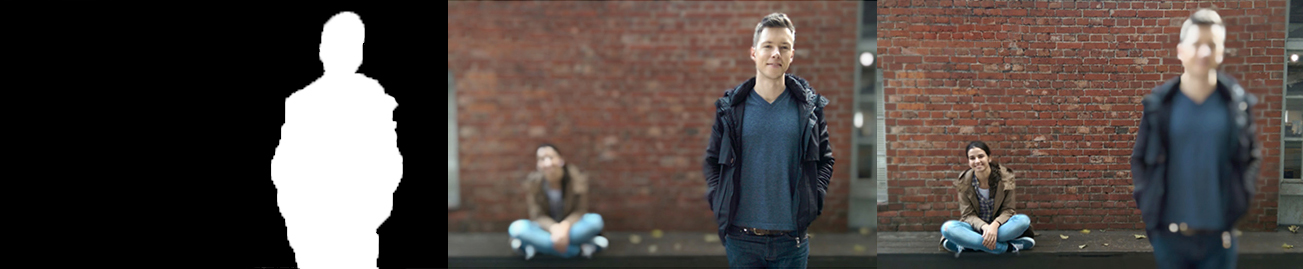
\includegraphics[width=\textwidth]{images/htc-ufocus.jpg}
\caption{HTC One M8 is capable of depth based image segmentation, which its UFocus\texttrademark\ technology uses to create a fake artistic bokeh.\label{figure:htc-ufocus} \cite{htc_one_ufocus}}
\end{figure}

Advancements in mobile camera technology have not only taken place in hardware but in software as well. In 2014 Apple, Android and Microsoft released new versions of their operating systems (iOS 8, Android 5.0 Lollipop and Windows Phone 8.1 respectively) all featuring, for the first time, APIs for manual camera control. In terms of functionality most modern smartphones will soon reach the level of high-end DSCs as features like fully manual exposure settings, RAW shooting and Optical Image Stabilization (OIS) are becoming increasingly more common. The boundaries of mobile camera technology are pushed further as media continues its convergence.

\section{Hybrid Mobile Applications}
\label{section:hybrid_mobile_landscape}

\subsection{The Landscape}
Mobile applications can be generally developed as native, hybrid or web applications. A native implementation offers the highest performance (least overhead) and the best access to the native device APIs (sensors, storage, contacts). However, building a mobile web application allows for better portability and code re-use across platforms and devices, which reduces development time and costs. Hybrid mobile applications (or, hybrid apps) combine the best of both worlds by leveraging web technologies to deploy native-like mobile applications to a broad range of smartphones. Hybrid apps can be further divided into \textit{WebView apps} and \textit{Compiled Hybrid apps}. WebView apps use web technologies (HTML, CSS and JavaScript) and the platform's native browser component (commonly known as the web view) to communicate with the platform's native layer. Compiled Hybrid apps on the other hand allow code written in one programming language to target multiple platforms by compiling it to platform-specific native code.

A widely popular tool for building \textit{WebView apps} is Apache Cordova\footnote{\url{https://cordova.apache.org/}}, an open-source cross-platform mobile development framework, originally known as PhoneGap and developed by Nitobi. After Adobe's acquisition of Nitobi in 2011 the PhoneGap codebase was contributed to the Apache Software Foundation to start the Apache Cordova project. Nowadays Adobe PhoneGap exists as a distribution of Apache Cordova including additional services such as Adobe PhoneGap Build and Adobe PhoneGap Enterprise. Since the release of Cordova in 2012 numerous commercial \textit{hybrid mobile development platforms} have emerged alongside Adobe's PhoneGap product line. Most notabe of these include products such as Telerik Platform, Ionic Platform, AppGyver Steroids, Sencha Touch, Trigger.io, Cocoon.io, Monaca and Intel XDK. They provide additional tooling (e.g. CLI programs and IDE plugins), generic UI components and SaaS/MBaaS services (e.g. storage, analytics and push notifications) to streamline the development and deployment of hybrid mobile applications for various platforms.

Unlike many of its commercial counterparts Cordova does not provide any readily available UI components or a client-side MVC framework. To cater for this need several UI frameworks optimized for hybrid mobile applications have been developed. These frameworks minimize development overhead by addressing common platform-specific browser quirks and by providing platform-specific styles and performance optimizations (e.g. removing the 300ms tap delay originally designed to help distinguish tap and scroll events in mobile browsers) \cite{click_delay}. Some of the more popular cross-platform mobile UI frameworks, the JavaScript libraries they depend on, and platforms they support are listed in Table \ref{table:cross-platform-mobile-ui-frameworks}.

\begin{table}[hb]
	\caption{Popular cross-platform mobile UI frameworks.} \label{table:cross-platform-mobile-ui-frameworks}

	\begin{center}
	\begin{tabular}{| m{3.05cm} | m{1.75cm} | m{2.75cm} | m{4.25cm} |}

		\hline
		\textbf{Framework}	&	\textbf{Released}		&		\textbf{Dependencies}		&	\textbf{Supported platforms}		\\ \hline
		React Native		&	03/2015						&	React						&	iOS, Android						\\ \hline
		Framework7 			&	04/2014						&								&	iOS, Android						\\ \hline
		Ionic				&	11/2013						&	AngularJS					&	iOS, Android						\\ \hline
		Onsen UI			&	09/2013						&	AngularJS					&	iOS, Android, WP8					 \\ \hline
		Kendo UI			&	11/2011						&	jQuery						&	iOS, Android, WP8					\\ \hline
		jQuery Mobile 		&	10/2010						&	jQuery						&	iOS, Android, WP8 \footnotesize{*}	\\ \hline

	\end{tabular}
	\end{center}
	\scriptsize{*} \small{platform-specific themes available as 3rd party extensions}
\end{table}

\subsection{WebView Applications}

Figure \ref{fig:web-view-app} provides a high-level overview of the architecture of a WebView application (henceforth referred to as WebView app). The example is based on Cordova's architecture, and as such, it is not fully representative of how related frameworks structure their applications. The general concepts are however similar as many of the frameworks are built on top of Cordova.

\begin{figure}[ht]
\centering 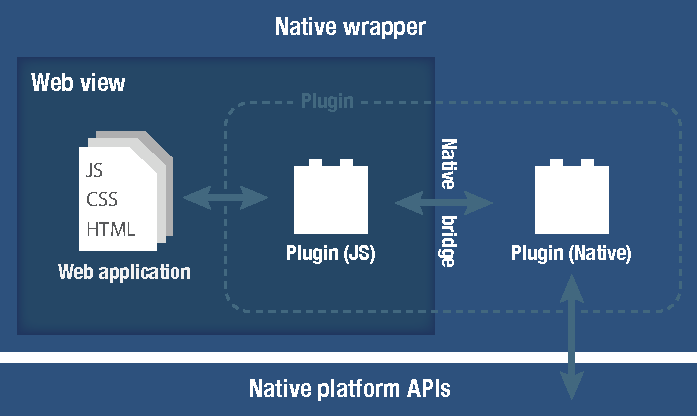
\includegraphics[width=\textwidth]{images/web-view-app-structure}
\caption{WebView app architecture; the application runs in a web view and communicates with the native platform APIs via a plugin interface.\label{fig:web-view-app}}
\end{figure}

WebView apps embed a web application into a native web view component running in a native application. The web application can hook into the native APIs by means of plugins (referred to as modules by some frameworks). The plugins consist of a non-native part written in JavaScript and a native part implemented in one or more platform-specific languages. Data between these two parts is passed as serialized JSON via a native bridge, a JavaScript-to-native interface defined by the framework. Most of the inherent overhead in WebView apps is caused by the message passing through the native bridge as a result of data serialization/deserialization and the layers of abstraction. In this regard WebView app plugins share similar characteristics to application servers that query remote APIs for data: they act as data providers that include a measurable query overhead (latency).

One of the culprits of WebView app development has been the lack of support for proper tooling --- a factor that led companies such as Facebook and LinkedIn to pick native over HTML5 for their mobile applications in 2012 and 2013, respectively \cite{html_vs_native_facebook}\cite{html_vs_native_linkedin}. In the past, due to the lack of proper support for debugging, developers had to resort to slow and brittle ways of littering their code with debug statements, which lead to slow feedback loops and cancelled out the main productivity benefit of hybrid application development: ``write once, run everywhere''. It was not until 2011 when the first 3rd party WebView app development tools, namely \textit{weinre} (WEb INspector REmote) and \textit{Apache Ripple}, emerged to address these issues. Powered by a feature-limited version of WebKit's (WK) Web Inspector, weinre allowed developers to remotely debug a web view running in a native application. Apache Ripple introduced the first browser-based cross-platform emulator allowing developers to quickly preview their WebView apps in the browser and avoid lengthy deployments to an emulator or a device.

Tooling for hybrid application development have seen significant improvement in the recent years. As browsers and mobile SDKs continue to mature, tools like weinre and Ripple have become legacy software. As of iOS 6.0 (released in late 2012) and Android 4.4 (released in late 2013) both iOS and Android smartphones ship with native support for remote debugging. As of this writing, weinre is still however the only viable option for remote debugging on some smaller platforms (most notably, Windows Phone). Most of Ripple's core functionality has been superseded by modern browsers that have introduced built-in support for various mobile device profiles and network simulation capabilities. Furthermore, emulators have become more efficient and are ever more suitable option for rapid debugging. Ripple might still however prove itself useful in legacy setups that run outdated SDKs or older browsers. Progress has also been made elsewhere in the industry as popular IDEs, such as Microsoft's Visual Studio and JetBrains' WebStorm, have integrated support for hybrid application development tools, and many hybrid mobile development platforms have developed new utilities to boost developer productivity. For example, with tools like \textit{PhoneGap Developer App} or \textit{Telerik AppBuilder Companion App} hybrid application developers are nowadays able to sync and preview their changes live on a device without a separate deployment.

While the improved tooling has tackled many of the early painpoints of WebView app development, the pitfalls of the underlying web view technology remain an issue. Regardless of the fact that the performance of web views has improved over the years and that it rarely raises issues for lightweight WebView apps, developers still need to account for \textit{device fragmentation}. Device fragmentation is an issue especially on Android, which as an open platform, allows vendors to introduce their own modifications to the OS software. Typically smartphone vendors ship updates to the smartphone's stock web view component on every major release. On Android however, as vendors are free to dictate which updates to apply, even phones running identical major OS versions are not guaranteed to have the exact same web view component. This causes issues for WebView app developers as the same target OS version might have different levels of support for certain web APIs and features.

Android addressed the fragmentation issue in its recent major release (Android 5.0) by decoupling the internal web view component into an \textit{updatable WebView}. Android phones running version 5.0 or later will no longer be subject to fragmentation as they are guaranteed to have an evergreen WebView that is independent of the OS update cycle. Developers targeting these newer Android  versions will however need to develop their WebView apps more like traditional web applications as updates to the WebView can potentially change (or break) existing web APIs at any time. To achieve a consistent target to develop against, hybrid application developers can leverage another emerging hybrid developemnt technology, namely Intel's Crosswalk. Crosswalk is open-source library that bundles a modified version of Chromium (an open-source runtime behind the Google Chrome browser) into the compiled Android application to work a replacement for the stock web view. It not only gives the developer a consistent web view (browser) to target, but also allows older Android phones (down until version 4.0) to benefit from the performance, security and feature updates of the newer Chromium. Crosswalk is becoming an integral part of many hybrid application development toolkits as evidenced by its recent integration to Cordova and commercial platforms like AppGyver Steroids, Ionic Platform and Intel XDK. With Crosswalk developers will, however, have to trade off better performance and consistency for increased application size (15-20MB) caused by the bundled Chromium runtime. An initiative within the Crosswalk developer community has been set forth to investigate ways to cut down the bundle size \cite{crosswalk_lite}.

\subsection{Compiled Hybrid Applications}

\textit{Compiled Hybrid applications}, or Compile Hybrid apps, target multiple platforms using a single programming language. They require less platform-specific code and offer better performance than WebView apps as the application is not run in a web view, but instead, transpiled into native code of the target platform. The trade-off is that Compiled Hybrid apps do not leverage web technologies to the same extent as WebView apps (in particular, web APIs and code re-usability). Compiled Hybrid apps strike a compromise between WebView apps and native applications in that UI and business logic are described in one common language as well as ``translated'' into corresponding native representation. Depending on the framework, translation could refer to either transpiling source code to native code or creating bindings from the source language to native methods.

One of the more popular \textit{cross-platform native frameworks} for developing Compiled Hybrid apps is Microsoft's Xamarin, which allows developing Android, iOS and Windows Phone applications using .NET technologies. Frameworks like Appcelerator Titanium and more recently released NativeScript and Facebook's React Native leverage JavaScript and common web development tools for the same effect. Unlike Xamarin, these frameworks do not transpile to native code, but rather use the platform's JavaScript engine -- for example, V8 on Android or JavaScriptCore on iOS -- to marshal method calls from JavaScript to the native side via predefined bindings. They leverage XML and a subset of CSS or their own implementation thereof to describe the UI. Platform-specific knowledge and code is required for implementing complex application and UI logic as the frameworks do not typically support all the APIs and UI components of the target platforms. Moreover, Compiled Hybrid app developers will be unable to take advantage of new APIs introduced by OS updates until the given framework implements the necessary bindings.

\subsection{Hybrid vs. Native}

The recent advancements in hybrid mobile development tooling and the emergence of new cross-platform native frameworks like NativeScript and React Native are indications of the growing interest towards hybrid mobile development. A hybrid approach is becoming an ever more viable not only because of the growing ecosystem but also because the average mobile developer targets an increasing number of platforms \cite{two_platforms}. Furthermore, the growing number of mobile web traffic originating from in-app browsers (web views) of popular applications like Facebook and Twitter has encouraged the vendors to reassess their web view component architecture: the most recent releases of iOS and Android introduced new web views (WKWebView and Chromium, respectively) whose performance is close on par with that of modern desktop browsers. \cite{souders_webview} Windows Phone is expected to follow suit with its upcoming Windows 10 OS and the new Edge browser engine \cite{spartan}. WebView app developers will soon be able to utilize the features of modern desktop browsers across all major mobile platforms.

As the hybrid mobile ecosystem continues to mature, the decision of choosing between a hybrid and a native approach to target multiple platforms becomes less obvious. Some of the factors to consider in such scenarios can be summarized as follows:

\begin{itemize}

	\begin{item}
	\textbf{Performance}: resource intensive mobile applications such as games benefit the most from a native implementation. While hybrid applications can leverage the Canvas and WebGL APIs to render graphics, the overhead of serializing user interactions over the native bridge is often too significant for any non-trivial game or graphics application. However, especially for modern smartphones a hybrid approach is still a very viable option if no real-time communication with the native level APIs is required.
	\end{item}

	\begin{item}
	\textbf{UI complexity}: Interactive applications featuring a complex UI and animations are best developed as native applications as hybrid frameworks typically support only a fixed set of UI components. Mimicking, or in other words re-implementing, platform-specific UI behaviour becomes less beneficial as the size and complexity of the UI grows.
	\end{item}

	\begin{item}
	\textbf{Development resources}: a hybrid approach allows developers with prior experience in web technologies to utilize their existing skill set in developing a (native) mobile application. Compiled Hybrid app developers will, however, often need to not only learn a new framework but also a new language. Companies with limited resources looking to target multiple platforms might find significant benefits in developing a WebView app, especially if they are looking to reuse code from their existing web applications.
	\end{item}

	\begin{item}
	\textbf{Portability}: fully native solutions have poor portability due to their platform specificity. WebView apps on the other hand allow existing web application code to be reused with minimal to moderate effort. Developers will however need to account for the fact that using a framework will force them to refactor any existing code to meet the conventions of that framework. For example, as seen in Table \ref{table:cross-platform-mobile-ui-frameworks}, developers that use the Ionic framework will need to structure their applications as per the architecture of AngularJS.
	\end{item}

\end{itemize}

\end{document}